%todo khepera, aibo vse na velka pismena Aibo, Khepera
\chapter{available software} \label{chap:software}
  in this chapter we shortly introduce software which helps programmer
  to debug and develop a program for a robot control. only simulators will be introduced, because 
  there is no available program or library for e-Puck like {\it Elib},
  which controls e-Puck remotely and asynchronously from pc.
  all introduced simulators run at pc and allow user to control and program a virtual copy of robot.
  most of the simulators simplify physics and construction, although they try to simulate sensors
  and actuators as faithfully as possible. some of the simulators support porting the program,
  which has been created for the virtual robot, to real robot.
  
\section{why simulators, why remote control?}
  {\it elib} and the simulators benefit from moving the debugging environment from the robot to pc.
  pc has enough resources at disposal and the code can be debugged much more comfortably. debugging
  tools depend on the structure of simulator and a programming language which is used by the simulator.
  {\it Elib} and the simulators allow to stop the program at any time.
  
  {\it Elib} uses $c\#$, which can be developed in Microsoft visual studio or Monodevelop studio.
  both studios support many features like setting breakpoints with conditions, call stack table,
  manual switching between threads and so on.
  
  the simulators have several advantages over robot remote control.
  a simulator provides the developer with a consistent behaviour of a virtual robot.
  a programmer has for example battery level under control. 
  the virtual robot measures in same situations identical values from its sensors. 
  
  The real robot is strongly influenced by the state of the battery
  and measures a completely different values in the same situation.
  Great advantage of the simulators is the possibility of not only stopping
  the running program, but also freezing the simulated environment. 
  
  Simulators also do not need a real robot for testing a program, which is extremely
  useful in the class with many students where only a few robots are available.
  Some of the simulators are completely free, which is certainly a nice quality.
  
  On the other hand, a remote control of a robot has some benefits too. 
  a lot of unpredictable situations are not simulated in simulators, although 
  many simulators have the option to involve randomness. the robot usually
  needs to be tested in the real environment too.
  
  Let us note, that simulators use physical and graphical engines. They are demanding applications
  for pc. 
  %todo rozvest co je fyzikalni engine? kde je to pouzivany v hrach, v simulatorech obejit napriklad citaci
  on the other hand, remote control is simple fast application.
  
  Last but not least, playing with real robot is simply much more entertaining. 	
  it motivates the users to solve real problems including hardware set up. 
  during programming a real robot the typical problems of mobile robotics are touch on.
  Simulators do not motivate the users to cope with a changing environment or an inaccurate odometry.
  
  In following subsections the simulators listed below will be discussed:
  \begin{itemize}
  \item Microsoft robotics developer studio\cite{msrs} is a complex tool based on message sending.
  \item Player/stage\cite{player} (gazebo) is an open source project developed in C++, which is widely used.
  \item Pyrobot(pyro)\cite{pyro} is also an open source project written in python. It supports abstract
  interfaces for devices convenient for e-Puck.
  \item Enki\cite{enki} is a fast simulation tool for a big population of robots.
  \item Commercial simulator webots\cite{webots} is the only simulator, which almost fully support e-Puck. 
  \end{itemize}
\section{Microsoft robotics developer studio\cite{msrs}} 
  microsoft robotics developer studio (msrs) is a set of tools including service-oriented runtime,
  simulator, visual programming language (vpl),
  tutorials and examples. msrs is based on .net and its runtime introduces following new technologies:
  \begin{itemize}
  \item concurrency and coordination runtime(ccr), which makes asynchronous programming easier.
  \item decentralised software services(dss) monitor services in real time for developers.
  \item common language runtime (clr) 2.0 is underlying runtime, 
          which interprets compiled code from any .net language.
  \end{itemize}	
  Msrs offers vpl, which is convenient for beginners or for building a structure of a new application.
  Vpl can be later easily transformed to any .net language.
  
  Visual simulation environment is based on ageia physx engine. It enables a 3D simulation.
  
  In general msrs is a rich set of tools, which introduce numerous nice features including
  technologies for easy asynchronous and concurrent programming. Especially ccr helps
  a programmer with concurrent programming. 
  
  There are enough tutorials for beginners written
  in $c\#$, visual basic or python. (iron python is an implementation of python for .net.)
  on the other hand, a lot of new features and tools bring a lot of new problems to users.
  Msrs tutorials and documentation have been rapidly improved in last year, but still some parts
  of the documentation are not easy accessible.
  
  Msrs runs only under Microsoft Windows operating systems and for a non commercial development
  it is for free. Neither e-Puck nor any similar robot is supported in the latest version of msrs.
  
  The studio would be a good solution for e-Puck, because it meets the requirements for {\it elib}.
  on the other hand, it is a huge, not portable, complicated environment.
  due to its complexity it discourages students from learning it.
\section{player/stage (gazebo) \cite{player}}
  player is a network server running on a robot and sending sensors values from the robot and
  accepting commands from clients. Player has a codified interface. Player translates
  commands from the interface to the implementation of actuators and translates values back from the robot sensors 
  to player interface. Unfortunately player is not implemented for e-Puck
  and for its devices.
  
  Stage is a 2D simulator, which is reflecting the sensors and actuators using the interface defined by player.
  It simulates a population of mobile robots and therefore it is possible to use player 
  in multi agent systems.
  The sensors are very simplified, because all sensors of the same type 
  have to implement the same interface. for example a sonar from Khephera and a sonar from Aibo robot
  has the same interface and stage treats them equally. 
  such simplification allows stage to be much quicker.
  
  Gasebo is a 3D simulator. Like stage gazebo simulates a big population of robots.
  It uses a rigid-body physics like stage too.
  
  The whole project is an open source and it is designed for posix-compatible systems.
  C/C++, python, java are the main supported languages.
  Player/stage is one of the most frequently used simulators in the research and is good for education purposes.
  A Khephera robot, which is similar to e-Puck is supported.
  It indicates, that it is worth to think about player/stage, if a simulator for e-Puck is wanted.
\section{pyrobot(pyro)\cite{pyro}}
  %\input{pyrobot_win.TpX}
  \begin{figure}
  \centering
  \ifpdf
    \setlength{\unitlength}{1bp}%
    \begin{picture}(323.15, 278.61)(0,0)
    \put(0,0){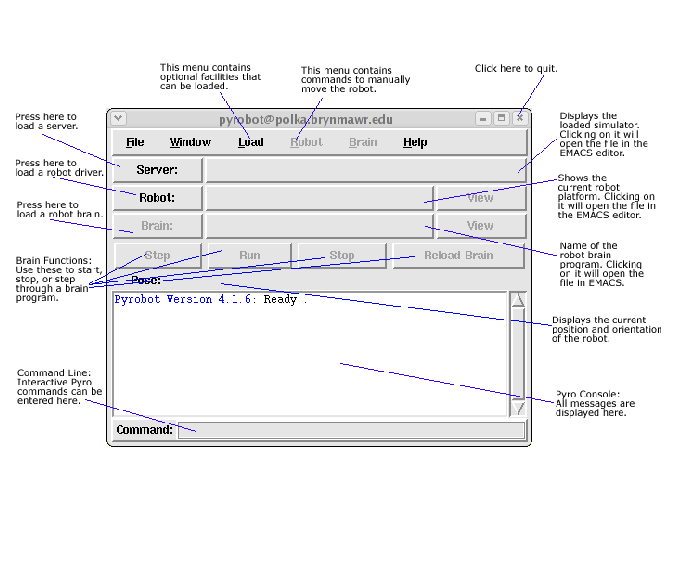
\includegraphics{pyrobot_win.pdf}}
    \end{picture}%
  \else
    \setlength{\unitlength}{1bp}%
    \begin{picture}(323.15, 278.61)(0,0)
    \put(0,0){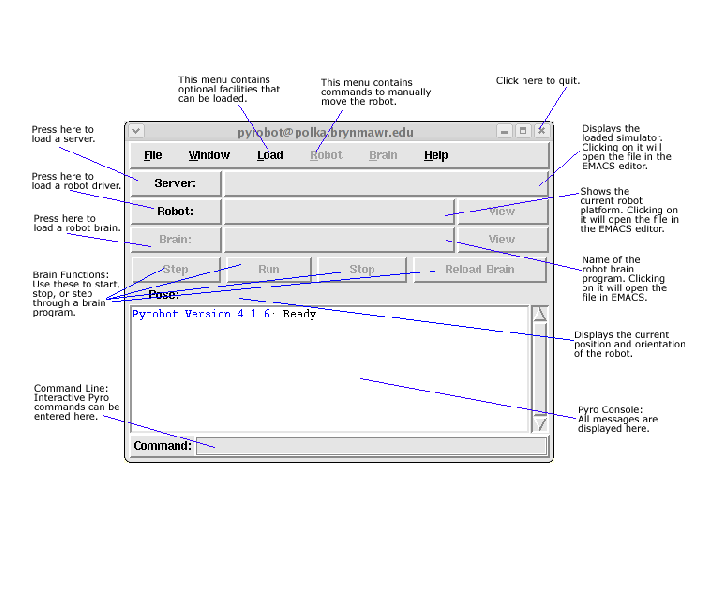
\includegraphics{pyrobot_win}}
    \end{picture}%
  \fi
  \caption{\label{pic:pyrobot_win}%
   Starting window of Pyrobot}
  \end{figure}



  Pyro is a shortcut from python robotics. It is an open source project written in python. Pyrobot is simulator
  from pyro project and the name pyrobot replaced the name of the project pyro. 
  Pyro abstracts interfaces of a robot and
  its devices, so each robot supported by pyro can be treated equally.
  pyro let a programmer choose from a list of simulators including player/stage, gazebo, pyrobot, khephera simulator
  and robocup soccer.
  After selecting a simulator there are available different worlds according to the selected simulator.
  A simulated robot can be driven from the command line or be controlled via loaded behaviour.
  
  The simulated robot can be easily replaced with real robot, if programs for controlling the real 
  and virtual robot are implemented. 	
  controlling the real robot is done via communication with program running on the robot similar 
  to {\it btcom} program on e-Puck.
  
  Khephera robot is supported. There is an implementation for e-Puck, which can simulate the robot
  and connect to the real robot, but the implementation does not support asynchronous operations and does 
  not implement all sensors and actuators.
  
  For using pyro as simulator for {\it elib} a translations between {\it btcom} and pyro protocol is needed.
  For more information see future works in conclusion ~\ref{chap:conclusion}.	
  
  Pyro project was abandoned in 2007 and no further development is planned.
  The advantage of the project is its portability due to the use of python and open source licence.
\section{enki \& aseba\cite{enki}}
  Enki is a library, which can simulate several robots hundred times faster than real time.
  The library is written in C++ and is still in development. It supports e-Puck including e-Puck's camera. 
  
  The e-Puck can be controlled via aseba. Aseba is a tool for robot control.
  It introduce a new scripting language. 
  the robots can be controlled only by the scripting language, which is the main
  drawback of enki, because the scripting language is very simple.
  In addition enki does not support the remote control of robots.
\section{webots\cite{webots}}
  
  %\input{webots_env.TpX}
  \begin{figure}
  \centering
  \ifpdf
    \setlength{\unitlength}{1bp}%
    \begin{picture}(223.94, 212.24)(0,0)
    \put(0,0){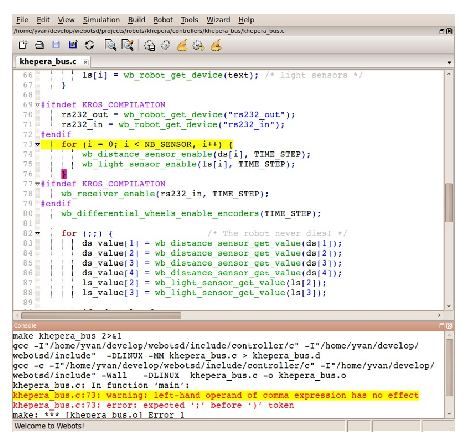
\includegraphics{webots_env.pdf}}
    \end{picture}%
  \else
    \setlength{\unitlength}{1bp}%
    \begin{picture}(223.94, 212.24)(0,0)
    \put(0,0){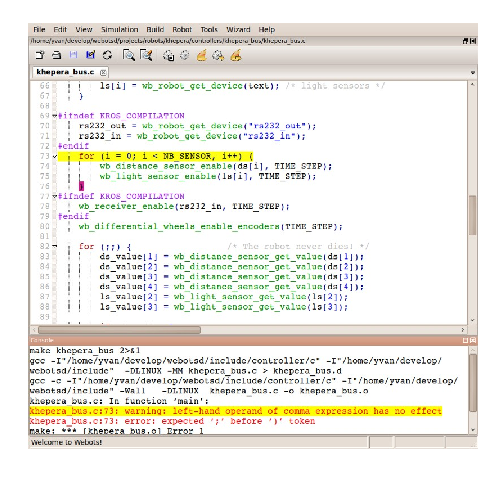
\includegraphics{webots_env}}
    \end{picture}%
  \fi
  \caption{\label{pic:webots_env}%
   Debuggin in Webots environment}
  \end{figure}

  webots is a simulation and prototyping tool for mobile robots.
  The simulation part will be described.  Prototyping tools allow to create a virtual robot,
  which will correspond to the real robot.
  Virtual e-Puck robot already has been designed
  by Webots's developers, so users of Webots do not have to design its own virtual robot, 
  which corresponds to real e-Puck.
  
  Development of a program under Webots is divided into four stages. 
  The first stage designing a virtual robot can be skipped,
  because the developers of Webots prepared for us finished virtual e-Puck as we mentioned.
  The second phase consists of programming robot in C language. 
  The third phase is the simulation. In the fourth stage a compiled program is flashed to e-Puck's memory.
  
  Webots has also the option of controlling e-Puck via Bluetooth.
  The robot can be programmed with graphical programming language for beginners or with C/C++ or Java,
  but only C/C++ can be compiled for the real e-Puck.
  
  The simulated worlds are created and saved in VRML and can be imported 
  from 3D Max, Cinema 4D.
  A lot of virtual worlds are already prepared, so it is not necessary to create them.
  
  Webots is a complex environment, in which it is easy to program, compile and load 
  a compiled hex file to e-Puck.
  The simulation runs in 3D and Webots supports all sensors and actuators except for microphones.
  A great advantage is that the real robot can be controlled by Bluetooth or
  programmed by loading a compiled program.
  Webots is also well documented and good tutorial are available.
  The significant drawback of Webots is its price and its annual fees.
  
  %\input{webots_sim.TpX}
  \begin{figure}
  \centering
  \ifpdf
    \setlength{\unitlength}{1bp}%
    \begin{picture}(206.93, 167.81)(0,0)
    \put(0,0){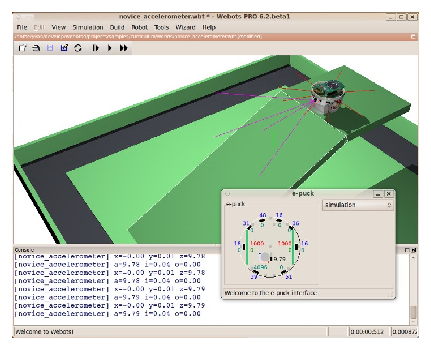
\includegraphics{webots_sim.pdf}}
    \end{picture}%
  \else
    \setlength{\unitlength}{1bp}%
    \begin{picture}(206.93, 167.81)(0,0)
    \put(0,0){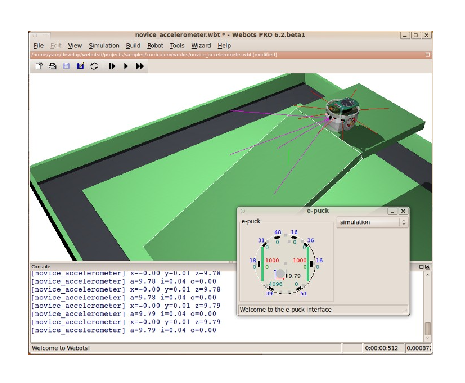
\includegraphics{webots_sim}}
    \end{picture}%
  \fi
  \caption{\label{pic:webots_sim}%
   Simulation of e-Puck behaviour}
  \end{figure}
